\documentclass[11pt]{article}
% Target: Data Mining and Knowledge Discovery (Springer). For submission, move this
% content into Springer Nature's sn-jnl template (sn-mathphys-ay or sn-basic style);
% the body uses only standard packages.
\usepackage[margin=1in]{geometry}
\usepackage{times}
\usepackage[hyphens]{url}
\usepackage{graphicx}
\usepackage[round]{natbib}
\usepackage{booktabs}
\usepackage{amsmath,amssymb}
\usepackage{array}
\usepackage{xcolor}
\usepackage[font=small]{caption}
\usepackage[colorlinks=true,linkcolor=blue!50!black,citecolor=blue!50!black,urlcolor=blue!50!black]{hyperref}
\setcounter{secnumdepth}{2}
\title{Chance Is the Wrong Baseline: Source-Prevalence Confounding in the Evaluation of Positive--Unlabelled Detectors, with Nominee Detection in the ICIJ Offshore Leaks Graph}
% CHECK: add co-authors and affiliations as appropriate.
\author{Joseph Bingham\\ Faculty of Biology, Technion -- Israel Institute of Technology\\ \texttt{jbingham@campus.technion.ac.il}}
\date{}
\begin{document}
\sloppy
\maketitle
\begin{abstract}
Node-level detectors of financial-secrecy enablers are trained and evaluated on
corpora pooled from heterogeneous sources, with positive--unlabelled (PU) labels
whose rate differs by source. We show that this design confounds both in-corpus
and cross-source evaluation, explain why, and give a protocol that corrects it. If
features identify an observation's source and the labelled rate differs across
sources, a model can score ``resembles a high-prevalence source'' instead of the
label. A within-source label permutation, which destroys label information but
keeps each source's rate, measures what this shortcut alone achieves. We derive the
population null score, predict when and in which direction it departs from $0.5$,
and confirm the prediction in a controlled simulation: the null moves only when
prevalence differs \emph{and} sources are separable, it falls below $0.5$ when the
signal points away from high-prevalence sources, pooled real-label scores are pulled
toward it, and source-balanced training restores both the null and the true effect.
On the full ICIJ Offshore Leaks graph (571{,}870 officers in four leaks) the
shortcut alone yields in-corpus AUCs of $0.63$--$0.68$ and leave-one-source-out
AUCs from $0.36$ to $0.69$; a source classifier predicts these nulls without any
permutation (correlation $0.98$, mean absolute error $0.02$). An apparent
below-chance ``inversion'' ($0.46$) sits $0.09$ above its null, and source-balanced
training lifts it to $0.69$. Across four leaks and seven finer sub-sources,
source-balanced transfer is $0.52$--$0.76$, honest in-corpus performance is
$0.67$--$0.81$ rather than the $0.72$--$0.83$ a pooled evaluation reports, and the
weak ``nominee'' label turns out to name companies almost exclusively. We
recommend reporting every pooled score next to its within-source permutation null,
and measuring transfer with source-balanced training.
\end{abstract}

\noindent\textbf{Keywords:} positive--unlabelled learning; evaluation methodology;
shortcut learning; permutation test; graph mining; offshore leaks


\begin{figure}[t]\centering
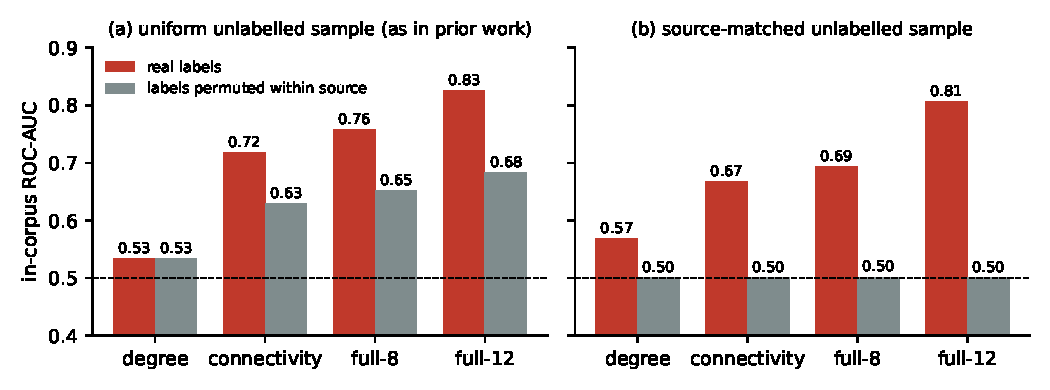
\includegraphics[width=0.92\textwidth]{fig_incorpus_null.pdf}
\caption{\textbf{In-corpus detection is partly source detection.} (a)~The usual
evaluation ranks held-out name-labelled nominees against a uniform sample of
unlabelled officers pooled across leaks. Permuting labels within each leak removes
all label information but keeps each leak's positive rate, and still yields
$0.63$--$0.68$. (b)~Drawing unlabelled officers with the same source composition as
the positives returns every permutation null to $0.50$; what remains ($0.57$--$0.81$)
is within-source signal. Bootstrap $95\%$ intervals are about $\pm0.01$.}
\label{fig:incorpus}\end{figure}

\section{Introduction}
Between 2013 and 2021 the International Consortium of Investigative Journalists
(ICIJ) released structured extracts of five leaks: Offshore Leaks, the Panama
Papers, the Bahamas Leaks, the Paradise Papers, and the Pandora Papers
\citep{icij}. Together they describe hundreds of thousands of shell companies, the
officers who nominally control them, the agents who incorporate them, and the
addresses where they are registered. The plumbing of offshore secrecy became a
graph one could compute on, and a natural question followed: can the professional
enablers of concealment be found automatically?

The usual formulation is node ranking. A concealed beneficial owner is, by design,
a structural dead end, but the enablers who stand in for owners are among the
busiest nodes in the graph, so they ought to be detectable. The seminal system in
this vein, SRBF, propagates suspiciousness from sanctions labels and reports
per-network AUROC between $0.69$ and $0.85$ \citep{srbf}. Labels are weak and
missing-not-negative, so the task is positive--unlabelled (PU) ranking
\citep{pusurvey}.

This paper is about how such detectors are evaluated. The ICIJ corpus is pooled
from sources that differ in jurisdiction, period, record-keeping, and what was
extracted, and a weak nominee label built from officer names is five times more
common in the Panama Papers than in the Paradise Papers. At the same time an
officer's structural features reveal which leak it came from. Together these two
facts create a shortcut: a model trained on the pooled corpus can raise the
scores of officers that \emph{look like} a high-prevalence source, and be rewarded
for it, without learning anything about nominees. The same mechanism produced
hospital-specific shortcuts in medical imaging, where a model learned the hospital
and the hospitals differed in disease prevalence \citep{zech2018variable}, and it
is a familiar form of shortcut learning \citep{geirhos2020shortcut}.

We measure the shortcut directly, by permuting labels within each source. The
permuted model has no access to which officers are nominees, only to how many
there are in each source. On the pooled in-corpus benchmark it scores $0.63$--$0.68$
(Fig.~\ref{fig:incorpus}a). Under leave-one-leak-out its held-out AUC ranges from
$0.36$ to $0.69$, depending on which leak is held out. Raw held-out AUCs are
therefore uninterpretable against chance. The Panama Papers, where every pooled
model appears to rank nominees \emph{below} random officers ($0.46$), is the leak
whose permutation null is lowest ($0.37$); a model that looks inverted is in fact
better than its null. The Paradise Papers, where transfer looks strong ($0.72$), has
a null of $0.69$.

We make five contributions. \emph{First}, we identify source-prevalence
confounding in pooled PU evaluation and quantify it with a within-source
permutation null, in-corpus and across sources (\S\ref{sec:res-incorpus},
\S\ref{sec:res-loo}). \emph{Second}, we derive the population null score, which
predicts when the null leaves $0.5$ and in which direction, and verify it in a
controlled simulation and on the real data, where a source classifier predicts all
twelve observed nulls to within $0.02$ on average (\S\ref{sec:mechanism}).
\emph{Third}, the simulation yields a diagnostic: comparing the pooled score, its
null, and a source-balanced score separates a shortcut-driven inversion from a
genuine reversal of the label--feature relationship, and only source-balanced
training recovers the effect size. \emph{Fourth}, on the ICIJ corpus, source-balanced
transfer is real but modest ($0.52$--$0.76$ across four leaks and seven
sub-sources), and the name-derived nominee proxy almost exclusively names
companies, whose share of the unlabelled pool varies from $20\%$ to $53\%$ across
leaks (\S\ref{sec:res-label}). \emph{Fifth}, we distil a four-part evaluation
protocol and apply it to a propagation ranker in the spirit of SRBF
(\S\ref{sec:protocol}, \S\ref{sec:res-srbf}).

The concern is general to computational social science. Public investigative
databases are not neutral social sensors; their labels and coverage inherit the
investigative and editorial processes that built them
\citep{compjourn,olteanu2019social}. When a corpus pools sources with different
base rates, a within-corpus score can measure the sources rather than the
phenomenon, and a detector can turn a source's record-keeping into an apparently
objective classification of people.

\section{Related Work}
\paragraph{Suspicious-node ranking on leaks.} SRBF \citep{srbf} ranks nodes in a
\emph{single} offshore network by connectivity propagated from sanctions labels.
We do not propose a better ranker; we ask what within- and cross-network scores
mean when sources are pooled, and apply our protocol to a propagation ranker in
the spirit of SRBF (\S\ref{sec:res-srbf}).
\paragraph{Graph learning for financial forensics.} A large literature applies
GNNs to \emph{transaction} graphs for anti-money laundering, most visibly on the
Elliptic Bitcoin dataset, where a random forest over node features was competitive
with graph convolutional networks \citep{aml}. Leak graphs encode ownership and
administrative roles rather than money flow, and strong non-graph baselines recur
in recent benchmarks \citep{graphland}, which motivates our gradient-boosting
models and structural nulls.
\paragraph{Shortcuts, confounding, and permutation tests.} Models exploit
features that predict the label in the training distribution without carrying
the intended construct \citep{geirhos2020shortcut}. When data are pooled across
sites that differ in prevalence, a model can learn the site; pneumonia detectors
learned which hospital a radiograph came from, and the hospitals differed in
disease prevalence \citep{zech2018variable}. Label-selection bias also induces
train/test shift on graphs \citep{shiftrobust}, and transductive success
overstates inductive generalisation \citep{graphuniverse}. Permutation tests are
standard for asking whether a classifier's score exceeds what label-independent
structure yields \citep{ojala2010permutation}; our contribution is to permute
\emph{within} source, so that the null keeps the source--prevalence structure that
creates the shortcut.
\paragraph{Provenance and annotation bias.} Biases enter social datasets at the
source and in processing \citep{olteanu2019social}; annotator identity and task
framing shape labels \citep{geva2019annotator}, sometimes in systematic,
group-linked ways \citep{sap2019racial}. Investigative data are an acute case
\citep{compjourn}, because the ``label'' is often a keyword rule or a journalistic
tag that was never designed for measurement.
\paragraph{Positive--unlabelled learning.} Under the assumption that positives are
labelled completely at random, treating unlabelled data as negative preserves the
ranking of the true posterior \citep{elkan}. The assumption is violated here in a
specific way: the labelling rate differs by source. Our permutation null measures
the consequence.

\section{Data and Task}\label{sec:data}
\subsection{Corpus and graph}
We use the public ICIJ Offshore Leaks CSV export (snapshot generated 9 September
2026; file checksums in the released code): $814$k entities, $771$k officers,
$3.34$M relationships. We build an undirected graph over \texttt{officer\_of},
\texttt{registered\_address}, and \texttt{intermediary\_of} edges ($2.01$M nodes,
$2.71$M edges), excluding record-resolution edges. For each officer we record its
entities through \texttt{officer\_of} edges whose sub-type is not a
beneficial-ownership role ($3.9\%$ of such edges are, and are excluded).
\subsection{Source assignment}\label{sec:sources}
Officers are assigned to a leak by the plurality source tag of their
\texttt{officer\_of} edges; every assigned officer draws all of its edges from a
single leak, because the same individual recurs across leaks as distinct nodes.
This yields a pool of $571{,}870$ officers in four leaks (Table~\ref{tab:data}).
Pandora edges and most Paradise registry edges carry no source tag, so this rule
drops them. Officer \emph{nodes} carry their own, finer tag (for example
``Paradise Papers -- Malta corporate registry''), which recovers the Barbados
registry ($127{,}891$ officers) and Pandora's service providers; we use node tags
for the sub-source analysis (\S\ref{sec:res-sub}).
\subsection{Labels}\label{sec:labels}
\emph{Name-derived proxy} ($14{,}878$ assigned officers): a case-insensitive match
of \textsc{nominee}, \textsc{nominees}, \textsc{trustee}, \textsc{fiduciar}, or
\textsc{nomini} in the officer name, an attribute no feature encodes.
\emph{Functional proxy} ($172$ officers, $155$ not name-matched): the nominee
endpoints of ICIJ's \texttt{underlying} edges (``Nominee Shareholder of'', etc.).
All $1{,}238$ source-tagged \texttt{underlying} edges are in Offshore Leaks, so the
functional label exists in one source only. We reserve ``nominee'' for the role
both proxies try to measure.
\subsection{Features and model}
Eight \emph{tabular} features per officer: entity degree and its logarithm; number
of the officer's own registered addresses; distinct intermediaries of its
entities; distinct entity jurisdictions; distinct \texttt{officer\_of} sub-types
(role diversity); entities per address; entities per intermediary. Four
\emph{graph} features: PageRank (damping $0.85$, 30 iterations), $k$-core number,
and mean and maximum neighbour degree. No feature encodes the name. The model is a
gradient-boosted tree ensemble (200 trees, depth 3, learning rate $0.1$);
tree ensembles are invariant to monotone per-feature transforms.

\begin{table}[t]\centering\small\setlength{\tabcolsep}{4pt}
\begin{tabular}{lrrrrr}
\toprule
leak & officers & name+ & prev. & corp.\,+ & corp.\,U\\
\midrule
Panama & 224{,}966 & 11{,}251 & 5.0\% & 0.98 & 0.53\\
Paradise & 217{,}418 & 1{,}969 & 0.9\% & 0.97 & 0.20\\
Offshore Leaks & 104{,}239 & 988 & 0.9\% & 0.99 & 0.20\\
Bahamas & 25{,}247 & 670 & 2.7\% & 0.37$^*$ & 0.50\\
\bottomrule
\end{tabular}
\caption{The four edge-assigned leaks. \emph{name+}: name-derived positives;
\emph{prev.}: their prevalence; \emph{corp.}: share of officer names carrying a
corporate suffix among positives (+) and unlabelled officers (U). $^*$Bahamas names
are truncated at 25 characters, which hides most suffixes. Panama supplies $76\%$
of all positives.}\label{tab:data}\end{table}

\section{Evaluation Protocol}\label{sec:protocol}
Four requirements, each aimed at a specific artifact (Table~\ref{tab:protocol}).
\paragraph{P1: a multi-type connectivity null.} A ``beyond degree'' claim must
beat a model on \{degree, address count, intermediary count\}, not degree alone.
\paragraph{P2: labels from an excluded attribute, with provenance characterised.}
The label should be built from an attribute absent from the features, and what it
actually names should be measured, not assumed.
\paragraph{P3: cross-source testing.} Train on $k\!-\!1$ sources and test on the
held-out one, ranking its positives against its own unlabelled officers.
\paragraph{P4: a within-source permutation null, source-balanced training, and source-matched sampling.}
Shuffle labels among the observations of each training source, keeping each
source's positive count, and rerun the identical pipeline; the resulting AUC is what
source membership alone buys. Report every pooled score next to its null, averaged
over enough draws to estimate it (its draw-to-draw s.d.\ here is $0.01$--$0.10$).
Measure the size of any transfer with source-balanced training, which removes the
shortcut. In-corpus, draw unlabelled observations with the same source composition
as the positives. Section~\ref{sec:mechanism} explains why each of these works.

\paragraph{Setup.} Training draws pair positives with unlabelled pseudo-negatives
at $1{:}3$. In-corpus evaluation uses a $70/30$ split of positives and ranks held-out
positives against $20$k fresh unlabelled officers, sampled uniformly (as in prior
work) or source-matched (P4). Leave-one-out evaluation ranks all positives of the
held-out source against up to $40$k of its unlabelled officers. We average over 5
(in-corpus) or 8 (leave-one-leak-out) training draws; permutation and sub-source
analyses use 3--4 draws. Confidence intervals pool $1{,}000$ bootstrap resamples of
the evaluation instances across draws. Because the unit of generalisation is the
source, these intervals describe ranking variability within a held-out source, not
variability across sources.

\begin{table}[t]\centering\small
\setlength{\tabcolsep}{5pt}\renewcommand{\arraystretch}{1.15}
\begin{tabular}{>{\raggedright\arraybackslash}p{2.3cm}>{\raggedright\arraybackslash}p{3.6cm}>{\raggedright\arraybackslash}p{4.4cm}>{\raggedright\arraybackslash}p{3.7cm}}
\toprule
requirement & artifact it prevents & diagnostic & finding on this corpus\\
\midrule
\textbf{P1} connectivity null & crediting degree as ``signal beyond degree'' & compare to a \{deg, addr, interm\} model & the null reaches $0.72$ in-corpus\\
\textbf{P2} excluded-attribute labels & learning the label's construction rather than the role & build labels from an unseen attribute; measure what they name & the name proxy names companies ($97$--$99\%$)\\
\textbf{P3} cross-source testing & mistaking one source's conventions for a portable signature & leave one source out & held-out AUC $0.46$--$0.76$\\
\textbf{P4} permutation null, balanced training & crediting source membership as detection & permute labels within source; source-balanced training; source-matched sampling & null $0.63$--$0.68$ in-corpus, $0.36$--$0.69$ held-out\\
\bottomrule
\end{tabular}
\caption{The protocol as a checklist. P4 is the addition that changes the reading
of every other number in this paper; Table~\ref{tab:diag} gives its diagnostic use.}\label{tab:protocol}\end{table}

\section{Results}\label{sec:results}

\subsection{In-corpus scores include source detection}\label{sec:res-incorpus}
Under the usual pooled evaluation, performance rises with model richness
(Table~\ref{tab:incorpus}): degree alone is near chance ($0.53$), the connectivity
null reaches $0.72$, the eight tabular features $0.76$, and adding graph features
$0.83$. With labels permuted within each leak, the same pipeline scores $0.63$,
$0.65$, and $0.68$ for the last three (Fig.~\ref{fig:incorpus}a). The mechanism is
simple. Panama supplies $76\%$ of the positives but $38\%$ of the unlabelled pool,
and the features identify an officer's leak: a classifier given only the eight
features recovers it with accuracy $0.72$ (random forest) or $0.70$ (logistic
regression), against $0.25$ chance. A model that learns ``looks like a Panama
officer'' is rewarded without learning anything about nominees.

Source-matched sampling removes this by construction. Every permutation null
returns to $0.50$ (Fig.~\ref{fig:incorpus}b), and the real-label scores fall to
$0.67$ (connectivity), $0.69$ (eight features), and $0.81$ (twelve features). Degree
\emph{rises}, from $0.53$ to $0.57$, because the pooled comparison had masked it.
Within-source signal is real, and higher-order features add the most of it, but
the pooled benchmark overstates the tabular models by $0.05$--$0.07$.

Two other checks matter less than expected. Grouping the train/test split by an
officer's dominant intermediary or address, so that co-located positives cannot
fall on both sides, changes the GBM figures by at most $0.015$
(Table~\ref{tab:incorpus}); co-location leakage is small for these models. And the
conclusions are unchanged across pseudo-negative ratios from $1{:}1$ to $1{:}10$
(in-corpus twelve-feature AUC $0.825$--$0.828$) and under bagging-PU training
\citep{mordelet2014bagging} ($0.760$ against $0.759$).

\begin{table}[t]\centering\small\setlength{\tabcolsep}{3.5pt}
\begin{tabular}{lcccc}
\toprule
& \multicolumn{2}{c}{uniform sample} & \multicolumn{2}{c}{source-matched}\\
\cmidrule(lr){2-3}\cmidrule(lr){4-5}
ranker & real & perm. & real & perm.\\
\midrule
degree & 0.534 & 0.534 & 0.568 & 0.501\\
connectivity null & 0.718 & 0.629 & 0.668 & 0.500\\
full-8 & 0.758 & 0.652 & 0.693 & 0.502\\
full-12 & 0.826 & 0.684 & 0.806 & 0.500\\
SRBF-inspired & 0.926 & -- & 0.913 & 0.496\\
\midrule
\multicolumn{5}{l}{\emph{split grouped by dominant intermediary (uniform sample)}}\\
full-12 / SRBF-inspired & 0.812 & & \multicolumn{2}{l}{/ 0.825}\\
\bottomrule
\end{tabular}
\caption{In-corpus detection of name-derived nominees. \emph{perm.}: labels
permuted within each leak. Uniform-sample, real-label 95\% bootstrap intervals are
about $\pm0.01$ (e.g.\ full-8 $[0.751, 0.769]$, full-12 $[0.818, 0.835]$).}
\label{tab:incorpus}\end{table}

\subsection{Cross-source scores must be read against their null}\label{sec:res-loo}
Table~\ref{tab:loo} and Fig.~\ref{fig:loo}a give leave-one-leak-out AUC for each
model and its within-source permutation null. Read against chance, the results
look erratic: the eight-feature model appears to invert on Panama ($0.459$, below
chance in $8/8$ draws, $95\%$ CI $[0.452, 0.465]$), the twelve-feature model on
Bahamas ($0.485$), and the eight-feature model appears to transfer well to
Paradise ($0.718$). Read against the null, the picture is consistent. The null
itself ranges from $0.36$ (Panama) to $0.69$ (Paradise), and the eight-feature
model exceeds it on every leak, by $+0.09$, $+0.03$, $+0.11$, and $+0.09$. The
twelve-feature model exceeds it on three of four ($+0.13$ to $+0.24$; Bahamas
$-0.02$). The ``inversion'' on Panama is a model that is better than its null on a
leak whose null sits far below chance. The excess over the null is a test, not an
effect size: the simulation in \S\ref{sec:mechanism} shows that pooled real-label
scores are pulled toward the null by an amount that depends on direction, so the
same true signal can show an excess of $+0.07$ or $+0.36$. The size of what
transfers is measured instead by source-balanced training (below).

Raw degree, which involves no training and so has no permutation null, transfers
at $0.50$--$0.61$, and higher-order features alone invert on Bahamas ($0.408$,
$8/8$ draws). A propagation ranker scores exactly $0.500$ on every held-out leak,
because with record-resolution edges excluded the leaks are disconnected
components and no personalised-PageRank mass reaches the held-out leak
(\S\ref{sec:res-srbf}).

\begin{table}[t]\centering\small\setlength{\tabcolsep}{3.2pt}
\begin{tabular}{lcccc}
\toprule
held-out leak & Panama & Paradise & Offshore & Bahamas\\
\midrule
raw degree (no training) & 0.576 & 0.499 & 0.614 & 0.544\\
connectivity: real & 0.436 & 0.538 & 0.548 & 0.544\\
\quad permutation null & 0.371 & 0.539 & 0.357 & 0.455\\
full-8: real & 0.459 & 0.718 & 0.642 & 0.576\\
\quad permutation null & 0.365 & 0.687 & 0.534 & 0.490\\
full-12: real & 0.601 & 0.719 & 0.656 & 0.485\\
\quad permutation null & 0.361 & 0.588 & 0.516 & 0.504\\
\midrule
full-8, source-balanced: real & 0.687 & 0.693 & 0.654 & 0.575\\
\quad permutation null & 0.534 & 0.439 & 0.533 & 0.465\\
full-8, per-source $z$-score & 0.685 & 0.651 & 0.668 & 0.571\\
full-8, per-source rank & 0.443 & 0.624 & 0.628 & 0.577\\
\bottomrule
\end{tabular}
\caption{Leave-one-leak-out ROC-AUC on the name-derived proxy, with the
within-source permutation null for each trained model (4 draws each; across-draw
s.d.\ $\le0.01$ for real labels, up to $0.05$ for most nulls and $0.10$ for the
balanced Panama null).}\label{tab:loo}\end{table}

\begin{figure}[t]\centering
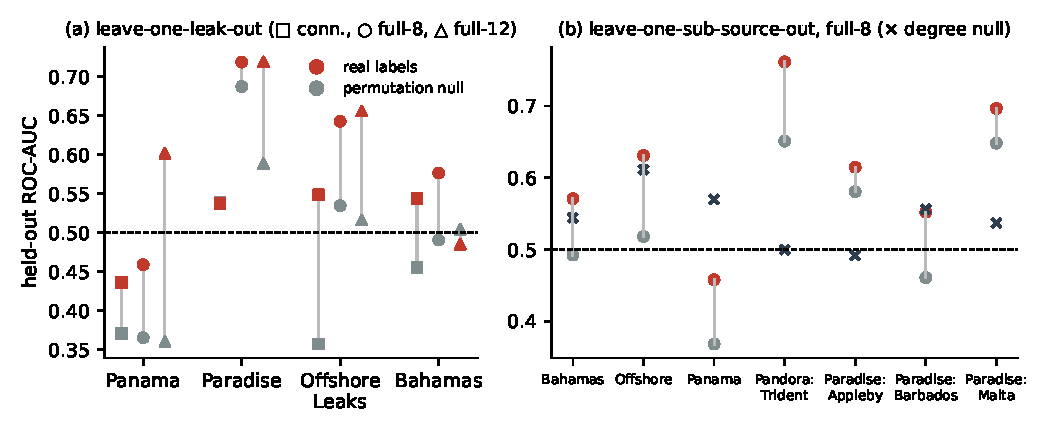
\includegraphics[width=0.92\textwidth]{fig_loo_null.pdf}
\caption{\textbf{Held-out AUC against its permutation null.} Red: real labels;
grey: labels permuted within each training source; the vertical line is the
excess over the null. (a)~Leave-one-leak-out for three models. The null ranges
from $0.36$ to $0.69$, so ``below chance'' and ``transfers well'' both misread the
data. (b)~Leave-one-sub-source-out with officer-node source tags, which adds the
Barbados registry and Pandora's Trident Trust. The eight-feature model beats its
null in all seven sub-sources, by $0.03$--$0.11$; crosses mark untrained raw
degree.}\label{fig:loo}\end{figure}

\paragraph{Removing the shortcut.} Training with equal positives and
pseudo-negatives per source removes the between-source prevalence difference.
The balanced nulls move toward chance ($0.44$--$0.53$, noisier because each source
contributes only $670$--$988$ positives), and real-label transfer becomes
$0.58$--$0.69$ with no inversion. Standardising each feature within its source
also removes the Panama inversion ($0.685$), but it is not a dependable fix: a
per-source rank transform does not ($0.443$), and per-source standardisation
\emph{creates} an inversion on Pandora's Trident Trust ($0.359$;
\S\ref{sec:res-sub}). Source-balanced training is the more reliable remedy, and
the permutation null is the check that it worked.

\paragraph{One reversal is genuine.} Not every below-chance score is the
shortcut. Trained on Offshore Leaks alone, where no between-source prevalence
difference exists, the model scores $0.456$ on Panama; every training set that
includes Offshore Leaks scores $0.44$--$0.46$, while Paradise alone ($0.680$) or
Paradise with Bahamas ($0.688$) transfer positively (Table~\ref{tab:subsets}).
The Panama result is thus the sum of a strong shortcut (null $0.36$--$0.42$ for
every multi-leak training set) and one genuine source-specific reversal. The
eight-feature profile of name-matched officers differs by leak
(Table~\ref{tab:smd}); in Panama they hold more registered addresses than other
officers (SMD $+0.69$; $87\%$ against $58\%$ have one), elsewhere about the same,
and dropping the address or intermediary count from the eight-feature model
lifts held-out Panama from $0.458$ to $0.573$ or $0.688$. A logistic-regression
model shows the same pattern ($0.461$ on Panama), so it is not specific to trees. By the diagnostic of \S\ref{sec:mechanism}, the pooled Panama
result (real $0.459$ above a null of $0.365$, balanced $0.687$) is a shortcut-driven
inversion, while the Offshore-trained result is a genuine reversal between two
sources.

\begin{table}[t]\centering\small\setlength{\tabcolsep}{4pt}
\begin{tabular}{lcc}
\toprule
training leaks (Panama held out) & real & perm.\ null\\
\midrule
Paradise & 0.680 & --\\
Offshore Leaks & 0.456 & --\\
Bahamas & 0.528 & --\\
Paradise + Bahamas & 0.688 & 0.359\\
Paradise + Offshore Leaks & 0.460 & 0.420\\
Offshore Leaks + Bahamas & 0.441 & 0.362\\
all three & 0.459 & 0.365\\
\bottomrule
\end{tabular}
\caption{Held-out Panama by training set (full-8). Single-source training has no
between-source prevalence difference to exploit; the null is defined only for
multi-source sets. The below-chance results track Offshore Leaks, not
pooling.}\label{tab:subsets}\end{table}

\begin{table}[t]\centering\small\setlength{\tabcolsep}{4.5pt}
\begin{tabular}{lrrrr}
\toprule
feature (SMD) & Panama & Parad. & Offsh. & Baham.\\
\midrule
entity degree & $+0.19$ & $+0.12$ & $+0.09$ & $+0.07$\\
address count & $+0.69$ & $+0.08$ & $-0.06$ & $-0.04$\\
interm.\ count & $+0.20$ & $+0.24$ & $+0.05$ & $-0.02$\\
role diversity & $-0.02$ & $-0.76$ & $-0.38$ & $-0.34$\\
\bottomrule
\end{tabular}
\caption{Standardised mean difference between name-derived positives and a random
sample of unlabelled officers, per leak (mean over 5 samples of $40$k). Only $0.1\%$
of Bahamas officers have any registered address.}\label{tab:smd}\end{table}

\subsection{Finer sources and Pandora}\label{sec:res-sub}
Four held-out leaks are a thin basis for a transfer claim. Officer-node tags
distinguish service providers and registries within a leak, and recover sources
the edge rule drops. Seven sub-sources have at least $2{,}000$ officers and $50$
name-matched positives (Table~\ref{tab:sub}). The eight-feature model, trained on
the other six and tested on each in turn, beats its permutation null in all seven,
by $+0.03$ (Appleby) to $+0.11$ (Offshore Leaks and Trident Trust)
(Fig.~\ref{fig:loo}b). Raw AUCs range from $0.46$ to $0.76$, and their order is
largely the order of the nulls: Trident Trust looks best ($0.761$) but its null is
$0.651$. With source-balanced training, transfer is $0.52$--$0.76$ and no
sub-source falls below chance; Panama rises from $0.458$ to $0.688$, and the
Barbados registry ($0.524$) is the one sub-source with essentially nothing to
transfer. The balanced nulls ($0.40$--$0.52$) are noisier than the pooled ones, since
six training sources each contribute only $553$ permuted positives and the held-out
positives differ strongly from their unlabelled officers, so any noise-fitted score
separates them in an arbitrary direction; three draws are a minimum here. Per-source standardisation helps Panama ($0.691$) and inverts Trident
($0.359$). With node tags, a five-leak design that includes Pandora gives
$0.517$--$0.775$ for the eight-feature model, with Panama falling below chance in
$3/4$ draws once Pandora and the Barbados registry join the training pool.

\begin{table}[t]\centering\small\setlength{\tabcolsep}{3pt}
\begin{tabular}{lrrcccc}
\toprule
sub-source & officers & pos. & real & null & bal. & bal.\ null\\
\midrule
Panama Papers & 224{,}966 & 11{,}251 & 0.458 & 0.368 & 0.688 & 0.523\\
Paradise: Barbados reg. & 127{,}891 & 580 & 0.552 & 0.461 & 0.524 & 0.501\\
Paradise: Malta reg. & 107{,}209 & 553 & 0.697 & 0.648 & 0.718 & 0.418\\
Offshore Leaks & 104{,}239 & 988 & 0.631 & 0.518 & 0.651 & 0.401\\
Paradise: Appleby & 72{,}406 & 1{,}388 & 0.615 & 0.581 & 0.660 & 0.490\\
Bahamas Leaks & 25{,}247 & 670 & 0.571 & 0.492 & 0.568 & 0.524\\
Pandora: Trident Trust & 3{,}692 & 710 & 0.761 & 0.651 & 0.757 & 0.428\\
\bottomrule
\end{tabular}
\caption{Leave-one-sub-source-out, full-8, officer-node source tags (3 draws).
\emph{real}/\emph{null}: pooled training and its within-source permutation null;
\emph{bal.}: source-balanced training (equal positives and $3\times$ pseudo-negatives
per training source) and its null.}\label{tab:sub}\end{table}

\subsection{What the label names}\label{sec:res-label}
\paragraph{The name proxy names companies.} Outside Bahamas, where names are
truncated, $97$--$99\%$ of name-matched officers carry a corporate suffix
(``\ldots\ Nominees Limited'', ``\ldots\ Trustees Ltd'', ``\ldots\ Trust Company as
Trustee of \ldots''); individual trustees are a small minority in every leak. The
unlabelled pool is not similarly uniform: $53\%$ of Panama's unlabelled officers
and $50\%$ of Bahamas' carry corporate names, against $20\%$ in Paradise and
Offshore Leaks (Table~\ref{tab:data}, Fig.~\ref{fig:labels}b). Structure separates
corporate from person-named officers well (source-matched AUC $0.82$ with eight
features, $0.88$ with twelve), so part of what a nominee detector detects is
``corporate officer'', and the payoff of doing so differs by source.

\paragraph{Among companies, the signal is local.} Restricting the unlabelled pool
to corporate-named officers asks the narrower question: which companies act as
nominees? Within source it is still answerable (source-matched in-corpus AUC
$0.74$ with eight features, $0.81$ with twelve; permutation null $0.50$). Across
leaks it is not: held-out AUC is $0.38$, $0.50$, $0.53$, and $0.53$, against nulls
of $0.27$, $0.48$, $0.45$, and $0.53$. Source-balanced training leaves Panama at
$0.377$, which by the diagnostic of \S\ref{sec:mechanism} is a genuine reversal: among
companies, what marks a nominee service in the other leaks marks the opposite in
Panama.

\paragraph{The functional label is a different population.} The $172$ functional
nominees are mostly small with a heavy tail (median entity degree $2$, mean
$318$, maximum $36{,}244$), whereas name-derived positives are almost all small
(median $1$, maximum $606$; Fig.~\ref{fig:labels}a). A model trained on the name
proxy ranks the $155$ name-independent functional nominees against other Offshore
Leaks officers at $0.55$ (eight features) and $0.35$ (connectivity null), while
untrained raw degree reaches $0.70$. Within the functional label, a connectivity
model separates held-out functional nominees at $0.92$ ($95\%$ CI $[0.87, 0.96]$,
$n\approx47$ per split). The functional nominees are structurally detectable; the
name-trained model has learned something else.

\begin{figure}[t]\centering
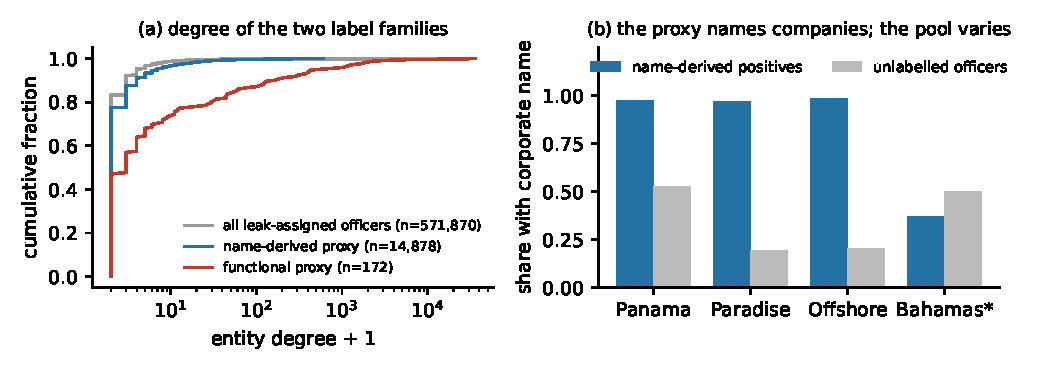
\includegraphics[width=0.92\textwidth]{fig_labels.pdf}
\caption{\textbf{The two label families.} (a)~Entity-degree ECDFs: name-derived
positives are almost all small; functional nominees have a heavy tail.
(b)~Corporate-suffix share among name-derived positives and unlabelled officers,
by leak; the proxy names companies everywhere, while the pool's corporate share
varies from $20\%$ to $53\%$. $^*$Bahamas names are truncated at 25
characters.}\label{fig:labels}\end{figure}

\subsection{A propagation ranker under the protocol}\label{sec:res-srbf}
We run a ranker in the spirit of SRBF \citep{srbf}: the stationary distribution of
a random walk with restart ($0.15$, 30 iterations) to the training positives over
the undirected graph. It is not a reimplementation of the original system.
In-corpus it scores $0.926$, survives source-matched sampling ($0.913$; null
$0.496$), and so is not a source shortcut. It is, however, partly co-location:
grouping the split by dominant intermediary lowers it to $0.825$, because a
held-out nominee that shares an intermediary with a training nominee receives
propagated mass. Across leaks it scores exactly $0.500$, because label propagation
cannot cross disconnected components. This does not apply to inductive models
with learned weights, such as a GNN trained on some sources and applied to
another, which we leave untested.

\subsection{Descriptive control}\label{sec:res-pos}
The enabler layer itself is real and extreme (Fig.~\ref{fig:hubs}): $358$
addresses register at least $100$ nodes ($30$ at least $1{,}000$; maximum
$37{,}338$), $729$ intermediaries incorporate at least $100$ entities ($90$ at least
$1{,}000$; maximum $35{,}358$), and the top $1\%$ of intermediaries account for
$63\%$ of intermediary--entity links ($35\%$ for addresses). Because these hubs are
defined by degree, finding them by degree is description rather than detection;
validating them against an external list of corporate service providers would make
it a detection result.

\begin{figure}[t]\centering
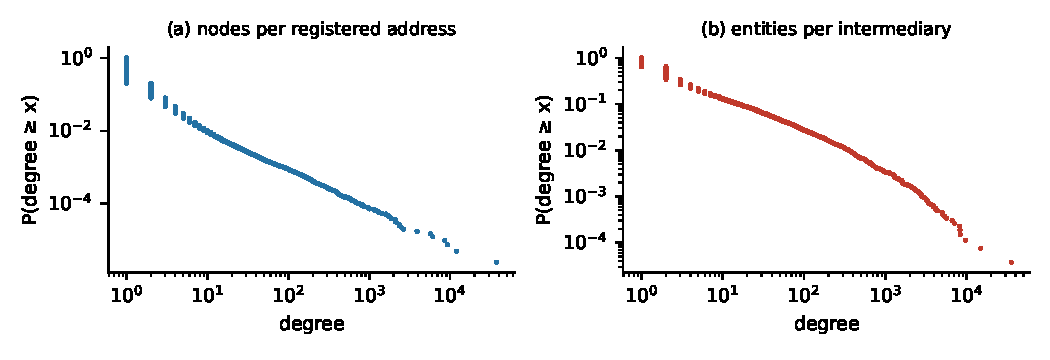
\includegraphics[width=0.92\textwidth]{fig_hubs.pdf}
\caption{The enabler layer is heavy-tailed (complementary CDFs, log--log): a few
addresses register tens of thousands of nodes and a few intermediaries incorporate
tens of thousands of entities.}\label{fig:hubs}\end{figure}

\section{Why the null moves: a model, a simulation, and a prediction}\label{sec:mechanism}

\subsection{The population null score}
Let training sources $s$ contribute $n_s$ observations with feature density $p_s$
and labelled-positive rate $\lambda_s$ (prevalence times labelling rate). Permuting
labels within each source keeps $\lambda_s$ and makes labels independent of
features within a source. The population-optimal score for the permuted problem is
then
\begin{equation}
P(\ell=1\mid x)=\sum_s \lambda_s\,P(s\mid x),\qquad P(s\mid x)=\frac{n_s p_s(x)}{\sum_{t} n_t p_t(x)},\label{eq:null}
\end{equation}
and sampling pseudo-negatives at a fixed ratio only applies a monotone transform,
so the permuted model ranks by $r(x)=\sum_s\lambda_s P(s\mid x)$. Its held-out AUC is
the probability that $r$ is larger for a labelled positive of the held-out source
than for one of its unlabelled observations. Three consequences follow.
(i)~If $\lambda_s$ is equal across training sources, $r$ is constant and the null is
$0.5$; source-balanced training enforces exactly this. (ii)~If $P(s\mid x)$ is
uninformative (sources not separable), the null is $0.5$. (iii)~Otherwise the null
is above $0.5$ when the held-out positives look more like high-$\lambda$ training
sources than its unlabelled observations do, and below $0.5$ when they look less
like them. To first order, if positives differ from unlabelled observations by a
shift $\beta w$ under isotropic noise, the null is approximately
$\Phi\big(\beta\,\langle\nabla r,w\rangle/(\sqrt2\,\lVert\nabla r\rVert)\big)$, with
$\nabla r$ taken at the held-out source's mean. In-corpus, pooled positives
over-represent high-$\lambda$ sources relative to a uniform unlabelled sample, so the
null exceeds $0.5$ whenever $\lambda_s$ varies and sources are separable;
source-matched sampling removes the imbalance and returns it to $0.5$.

\subsection{Simulation}
We simulate four sources in $\mathbb{R}^8$ with identity covariance: a held-out
target $T$ at the origin and training sources $H$, $A$, $B$ at distance $\delta$
along three axes. Prevalence is $\pi_0=0.03$ in $T$, $A$, $B$ and $\rho\pi_0$ in $H$;
positives are shifted by $\beta w$, with $w$ at angle $\theta$ to the axis of $H$
and otherwise orthogonal to all source offsets; each positive is labelled with
probability $0.5$. Each source has $20{,}000$ observations, and the pipeline is the
paper's (gradient boosting of depth 3, $1{:}3$ pseudo-negatives, ten replicates per
setting). Figure~\ref{fig:sim} and Table~\ref{tab:sim} summarise the results.

\emph{When the null moves.} With equal prevalence ($\rho=1$) the held-out null stays
at $0.48$--$0.50$ whatever the separation; with separation and unequal prevalence
it falls to $0.34$--$0.45$ at $\theta=180^\circ$ (Fig.~\ref{fig:sim}a). The
population prediction is more extreme ($0.28$--$0.30$) than the fitted null, because
a finite model estimates $P(s\mid x)$ imperfectly and shrinks toward $0.5$. One
setting departs from the formula in an instructive way: with no separation
($\delta=0$) but $\rho=8$, the null is $0.60$, because $H$'s many positives are the
only thing distinguishing it, so ``resembles $H$'' then means ``resembles a
positive''. In-corpus, the uniform-sample null rises to $0.70$, while the
source-matched null stays at $0.49$--$0.51$ in every setting.

\emph{Direction.} At $\rho=4$, $\delta=1$, $\beta=1$, the null moves from $0.68$
($\theta=0^\circ$, signal toward $H$) through $0.51$ ($90^\circ$) to $0.36$ ($180^\circ$),
tracking the population prediction (Fig.~\ref{fig:sim}b). The true within-target
AUC is about $0.76$ throughout. The pooled real-label score is pulled toward the
null ($0.75$ to $0.71$), so the excess over the null ranges from $+0.07$ to $+0.36$
for the same signal: it is a valid test for signal beyond the shortcut but not an
effect size. Source-balanced training recovers the true AUC at every angle
($0.73$--$0.74$), and its null stays at $0.49$--$0.51$. With no signal ($\beta=0$),
every quantity is at $0.49$--$0.53$.

\emph{Genuine reversal.} If the signal's sign is flipped in the target, the pooled
score falls \emph{below its null} ($0.27$ against $0.49$ at $\beta=1$), and
source-balanced training stays below chance ($0.27$). A shortcut-driven inversion
looks different: the pooled score is below $0.5$ but above its null, and
source-balanced training lifts it above $0.5$. Table~\ref{tab:diag} turns this into
a diagnostic.

\begin{figure}[t]\centering
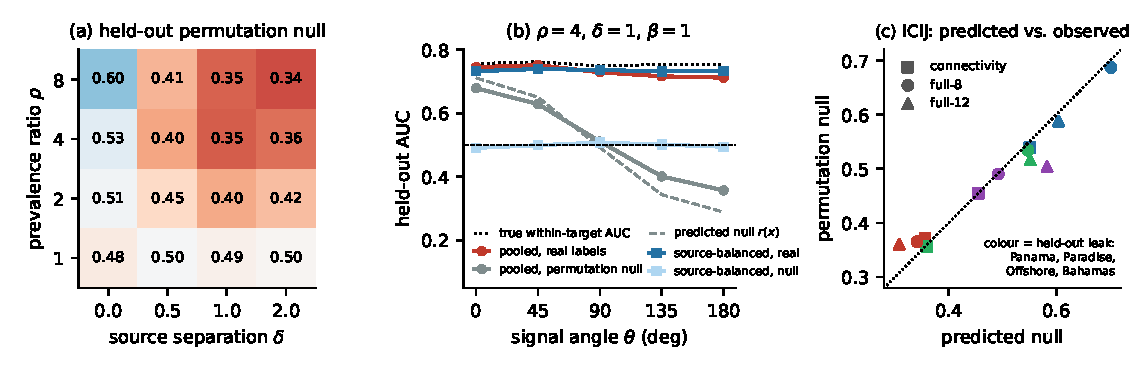
\includegraphics[width=\linewidth]{fig_sim.pdf}
\caption{\textbf{The null score, simulated and predicted.} (a)~Held-out permutation
null as a function of prevalence ratio $\rho$ and source separation $\delta$
($\theta=180^\circ$, $\beta=1$, ten replicates). (b)~Direction sweep: the
null follows the population prediction $r(x)$; pooled real-label scores are pulled
toward it; source-balanced training recovers the true within-target AUC (dotted)
and its null stays at $0.5$. (c)~On the ICIJ corpus, the null predicted from a
source classifier through Eq.~\eqref{eq:null}, with no permutation, matches the
twelve observed permutation nulls (correlation $0.98$).}\label{fig:sim}\end{figure}

\begin{table}[t]\centering\small\setlength{\tabcolsep}{4pt}
\begin{tabular}{lcccccc}
\toprule
setting & real & null & pred.\ null & bal. & bal.\ null & true\\
\midrule
$\rho=1$, $\delta=1$, $\theta=180^\circ$ & 0.729 & 0.488 & 0.500 & -- & -- & --\\
$\rho=8$, $\delta=2$, $\theta=180^\circ$ & 0.530 & 0.338 & 0.291 & -- & -- & --\\
$\rho=4$, $\delta=1$, $\theta=0^\circ$ & 0.745 & 0.678 & 0.711 & 0.732 & 0.491 & 0.756\\
$\rho=4$, $\delta=1$, $\theta=90^\circ$ & 0.729 & 0.511 & 0.492 & 0.736 & 0.508 & 0.748\\
$\rho=4$, $\delta=1$, $\theta=180^\circ$ & 0.712 & 0.357 & 0.289 & 0.734 & 0.494 & 0.754\\
reversed in target, $\theta=90^\circ$ & 0.270 & 0.493 & -- & 0.266 & -- & 0.246\\
\bottomrule
\end{tabular}
\caption{Selected simulation settings ($\beta=1$; ten replicates; replicate s.d.\ of
the nulls $0.02$--$0.04$). \emph{pred.\ null}: population score $r(x)$ of
Eq.~\eqref{eq:null}; \emph{true}: AUC of the true signal direction in the target.}
\label{tab:sim}\end{table}

\begin{table}[t]\centering\small\setlength{\tabcolsep}{4pt}
\begin{tabular}{p{3.6cm}p{2.3cm}p{2.3cm}p{4.2cm}}
\toprule
pattern & pooled vs.\ null & balanced & reading\\
\midrule
no signal beyond the shortcut & real $\approx$ null & $\approx0.5$ & nothing transfers\\
shortcut masks a real signal & real $>$ null, real can be $<0.5$ & $>0.5$ & signal transfers; report the balanced score\\
genuine reversal & real $<$ null & $<0.5$ & the label--feature relation flips across sources\\
\bottomrule
\end{tabular}
\caption{Reading a cross-source score with P4. On the ICIJ corpus, pooled Panama is
the second pattern (real $0.459$, null $0.365$, balanced $0.687$); companies-only
Panama is the third (balanced $0.377$).}\label{tab:diag}\end{table}

\subsection{Predicting the observed nulls}
Equation~\eqref{eq:null} can be evaluated on real data without permuting anything:
train a source classifier on the training leaks, re-weight its posteriors to the
pool's source composition, weight them by each source's label rate, and score the
held-out leak. For the four held-out leaks and three feature sets, the predicted
nulls match the observed permutation nulls with correlation $0.98$ and mean absolute
error $0.02$ (Fig.~\ref{fig:sim}c); for example, eight features give predicted
$0.34$, $0.70$, $0.55$, $0.49$ against observed $0.37$, $0.69$, $0.53$, $0.49$. The
largest miss is Bahamas with twelve features ($0.58$ against $0.50$). The confound in
\S\ref{sec:res-incorpus}--\ref{sec:res-loo} is therefore this mechanism, and a
practitioner can anticipate a null before computing it.

\section{Discussion}\label{sec:disc}
The central finding is methodological. When a PU corpus pools sources whose label
rates differ and whose features identify the source, both in-corpus and
cross-source AUC mix detection with source membership, in proportions that vary
by source and can push a score above or below chance. Equation~\eqref{eq:null}
says when this happens and in which direction, the simulation confirms it, and on
the ICIJ corpus the predicted nulls match the observed ones. The effect is large
here: the shortcut alone is worth $0.63$--$0.68$ in-corpus, and held-out nulls range
from $0.36$ to $0.69$. Neither of the two stories one might tell from raw numbers
(``detection inverts'' or ``detection transfers well'') survives comparison with
the null. What survives is modest: source-balanced transfer of $0.52$--$0.76$, real
within-source signal ($0.67$--$0.81$ with source-matched sampling), and genuine
reversals between Offshore Leaks and Panama and, among companies, between Panama
and the other leaks.

The mechanism is not specific to offshore leaks. It applies whenever labelled data
are pooled from sources that differ in label rate and are identifiable from the
features: fraud and anti-money-laundering data pooled across institutions,
clinical cohorts pooled across hospitals \citep{zech2018variable}, or moderation
labels pooled across platforms. In each case the within-source permutation null is
cheap to compute and, as Eq.~\eqref{eq:null} shows, can even be predicted in advance
from a source classifier.

The label analysis explains part of why transfer is small. The name proxy picks out
corporate nominee and trustee services in every leak, so ``nominee'' and
``corporate officer'' are entangled, and the corporate share of the comparison
pool differs by leak. Among companies, what distinguishes nominee services from
other corporate officers is source-specific. The functional label, which comes
from one source, describes a different and more connected population, and a
name-trained detector does not find it.

\paragraph{Implications for practice.} For detection on pooled data: report a within-source permutation null alongside
every in-corpus and cross-source score, with its draw-to-draw spread; treat the
excess over the null as a test, and measure transfer with source-balanced training;
in-corpus, sample unlabelled observations to match the positives' source
composition; prefer source-balanced training to feature normalisation, and verify
it with the null; use Table~\ref{tab:diag} to tell a shortcut-driven inversion from a
genuine reversal; measure what a keyword label actually
names before treating it as ground truth; and prefer descriptive, label-free hub
analytics when the goal is to map the enabler layer rather than to classify
individuals. Each of these is cheap, and P4 alone would have changed the reading
of every number in prior within-corpus evaluations on this corpus.

\section{Limitations}
The cross-source analysis rests on the name-derived proxy, because the functional
label exists in one source; its small size ($155$) makes within-label intervals
wide. Our corporate-name rule is a suffix heuristic and fails on Bahamas' truncated
names; we have not manually audited label matches, which would quantify the
proxy's precision per source. The permutation null captures shortcuts that run
through the source's positive rate; it does not capture every form of shift, and
excess over the null is a test rather than an effect size. Our derivation of the
null is a population argument; the first-order formula assumes a shift model and
isotropic noise, and the simulation uses Gaussian sources, so the magnitudes it
reports are illustrative while the qualitative regimes are general. Source-balanced
training discards data from large sources and its null is noisier; with few
positives per source, more draws are needed.
Seven sub-sources is still a modest number of domains, and our models are
representative rather than exhaustive: an inductive multi-relational GNN under the
same protocol remains future work. Features are computed on the full graph, so the
held-out source's structure is available at test time; our cross-source tests are
transfer tests rather than strictly inductive ones. Finally, partial extraction
leaves the true prevalence of nominees unknowable, so all metrics are PU lower
bounds on how well any ranking matches the role.

\section{Ethics and reproducibility}
All data are drawn from the public ICIJ database, which records companies, roles,
and addresses; appearance in the leaks is not evidence of wrongdoing. We make no
attempt to de-anonymise concealed owners or to attribute wrongdoing to named
individuals. Because a detector treated as reliable could wrongly flag a named
person or firm, and our results show that within-corpus scores overstate what
such detectors know, we caution against individual-level use, and any release
should avoid producing ready-to-use ranked lists of named entities.

For reproducibility: the name label is the case-insensitive pattern
\texttt{NOMINEE|NOMINEES|TRUSTEE|FIDUCIAR|NOMINI}; beneficial-ownership sub-types
are \texttt{officer\_of} links matching \texttt{beneficial|beneficiary}; role
sub-types are lower-cased with a trailing ``of'' removed. The model is scikit-learn's
histogram gradient boosting (200 iterations, depth 3, learning rate $0.1$, no early
stopping). Every number in this paper is produced by released scripts run directly
on the public CSV export; the snapshot date and SHA-256 checksums of each file are
recorded with the code. All experiments run on a single CPU core with under 4\,GB
of memory; the full battery takes about an hour. The ICIJ database is used under
its published terms; we introduce no new dataset and release only analysis code.


\section{Conclusion}
Nominee detection on the ICIJ corpus looks strong within the corpus and erratic
across it, and both impressions are partly produced by the same thing: sources that
differ in label rate and are identifiable from structure. The population null score
explains when this happens and in which direction, a simulation confirms it, and a
source classifier predicts the observed nulls on the real data. Against the null,
and with source-balanced training, out-of-source signal is real but modest,
within-source signal is real once source-matched sampling removes the shortcut,
and the name-derived label names companies. On pooled data, an AUC is not yet
evidence of detection until it has been compared with what the source alone would
have scored.

\section*{Declarations}
% CHECK: complete every item below for the DMKD submission system.
\paragraph{Funding.} [To be completed by the authors.]
\paragraph{Competing interests.} The authors declare no competing interests. % CHECK
\paragraph{Data availability.} The ICIJ Offshore Leaks Database is publicly
available from \url{https://offshoreleaks.icij.org}; we used the CSV export generated
on 9 September 2026, whose file checksums are recorded with the code.
\paragraph{Code availability.} All code used to produce the results, tables, and
figures, including the simulation, is available at [repository URL]. % CHECK
\paragraph{Author contributions.} [To be completed by the authors.]
% CHECK: describe accurately how the model was used in this version and which versions.
\paragraph{Use of generative AI.} A large language model (Claude, Anthropic) was used
to rebuild and run the analysis pipeline and simulation from the authors'
specification, to prepare figures, and to draft and revise text. The authors
designed the study, checked the code and results, and take responsibility for all
claims.

% CHECK: references were added without access to a search tool; verify every entry.
\begin{thebibliography}{Van Langendonck et al.(2025)}
\providecommand{\natexlab}[1]{#1}

\bibitem[Bazhenov et al.(2025)]{graphland}
G.~Bazhenov, O.~Platonov, and L.~Prokhorenkova.
\newblock {GraphLand}: Evaluating Graph Machine Learning Models on Diverse
  Industrial Data.
\newblock In \emph{Advances in Neural Information Processing Systems (NeurIPS)},
  2025.

\bibitem[Bekker and Davis(2020)]{pusurvey}
J.~Bekker and J.~Davis.
\newblock Learning from positive and unlabeled data: a survey.
\newblock \emph{Machine Learning}, 109:719--760, 2020.

\bibitem[Cohen et al.(2011)]{compjourn}
S.~Cohen, J.~T.~Hamilton, and F.~Turner.
\newblock Computational Journalism.
\newblock \emph{Communications of the ACM}, 54(10):66--71, 2011.

\bibitem[Elkan and Noto(2008)]{elkan}
C.~Elkan and K.~Noto.
\newblock Learning classifiers from only positive and unlabeled data.
\newblock In \emph{Proc.\ ACM SIGKDD (KDD)}, pp.~213--220, 2008.

\bibitem[Geirhos et al.(2020)]{geirhos2020shortcut}
R.~Geirhos, J.-H.~Jacobsen, C.~Michaelis, R.~Zemel, W.~Brendel, M.~Bethge, and
  F.~A.~Wichmann.
\newblock Shortcut learning in deep neural networks.
\newblock \emph{Nature Machine Intelligence}, 2(11):665--673, 2020.

\bibitem[Geva et al.(2019)]{geva2019annotator}
M.~Geva, Y.~Goldberg, and J.~Berant.
\newblock Are We Modeling the Task or the Annotator? An Investigation of Annotator
  Bias in Natural Language Understanding Datasets.
\newblock In \emph{Proc.\ EMNLP-IJCNLP}, 1161--1166, 2019.

\bibitem[ICIJ(2024)]{icij}
International Consortium of Investigative Journalists.
\newblock The {ICIJ} Offshore Leaks Database. Continuously updated database;
  snapshot of 9 September 2026.
\newblock \url{https://offshoreleaks.icij.org}.

\bibitem[Joaristi et al.(2019)]{srbf}
M.~Joaristi, E.~Serra, and F.~Spezzano.
\newblock Detecting suspicious entities in Offshore Leaks networks.
\newblock \emph{Social Network Analysis and Mining}, 9(1):62, 2019.

\bibitem[Mordelet and Vert(2014)]{mordelet2014bagging}
F.~Mordelet and J.-P.~Vert.
\newblock A bagging {SVM} to learn from positive and unlabeled examples.
\newblock \emph{Pattern Recognition Letters}, 37:201--209, 2014.

\bibitem[Ojala and Garriga(2010)]{ojala2010permutation}
M.~Ojala and G.~C.~Garriga.
\newblock Permutation tests for studying classifier performance.
\newblock \emph{Journal of Machine Learning Research}, 11:1833--1863, 2010.

\bibitem[Olteanu et al.(2019)]{olteanu2019social}
A.~Olteanu, C.~Castillo, F.~Diaz, and E.~K{\i}c{\i}man.
\newblock Social Data: Biases, Methodological Pitfalls, and Ethical Boundaries.
\newblock \emph{Frontiers in Big Data}, 2:13, 2019.

\bibitem[Sap et al.(2019)]{sap2019racial}
M.~Sap, D.~Card, S.~Gabriel, Y.~Choi, and N.~A.~Smith.
\newblock The Risk of Racial Bias in Hate Speech Detection.
\newblock In \emph{Proc.\ ACL}, 1668--1678, 2019.

\bibitem[Van Langendonck et al.(2026)]{graphuniverse}
L.~Van Langendonck, G.~Bern\'ardez, N.~Miolane, and P.~Barlet-Ros.
\newblock {GraphUniverse}: Synthetic Graph Generation for Evaluating Inductive
  Generalization.
\newblock In \emph{International Conference on Learning Representations (ICLR)},
  2026.

\bibitem[Weber et al.(2019)]{aml}
M.~Weber, G.~Domeniconi, J.~Chen, D.~K.~I.~Weidele, C.~Bellei, T.~Robinson, and
  C.~E.~Leiserson.
\newblock Anti-Money Laundering in Bitcoin: Experimenting with Graph
  Convolutional Networks for Financial Forensics.
\newblock In \emph{KDD Workshop on Anomaly Detection in Finance}, 2019.

\bibitem[Zech et al.(2018)]{zech2018variable}
J.~R.~Zech, M.~A.~Badgeley, M.~Liu, A.~B.~Costa, J.~J.~Titano, and E.~K.~Oermann.
\newblock Variable generalization performance of a deep learning model to detect
  pneumonia in chest radiographs: a cross-sectional study.
\newblock \emph{PLOS Medicine}, 15(11):e1002683, 2018.

\bibitem[Zhu et al.(2021)]{shiftrobust}
Q.~Zhu, N.~Ponomareva, J.~Han, and B.~Perozzi.
\newblock Shift-Robust {GNN}s: Overcoming the Limitations of Localized Graph
  Training Data.
\newblock In \emph{NeurIPS}, 2021.

\end{thebibliography}

\end{document}
